
\section{Heavy flavour process in \znunu+jets}
\label{sec:zplusbb_app}

To investigate the effects of heavy flavour process on \znunu+jets 
background estimation, the cross section for heavy flavour process, 
defined as events with at least one bjets in generator level, is varied 
with a factor of 0.5 and 2 separately in the likelihood for the 
validation of \nb modelling. The effects are accessed by inspecting 
changes on the btag nuisances. Figure~\ref{fig:zplusbb} shows the effects 
on btag nuisances from the heavy flavour process are less than 1 sigma pull.
\par

\begin{figure}[h!]
  \centering
  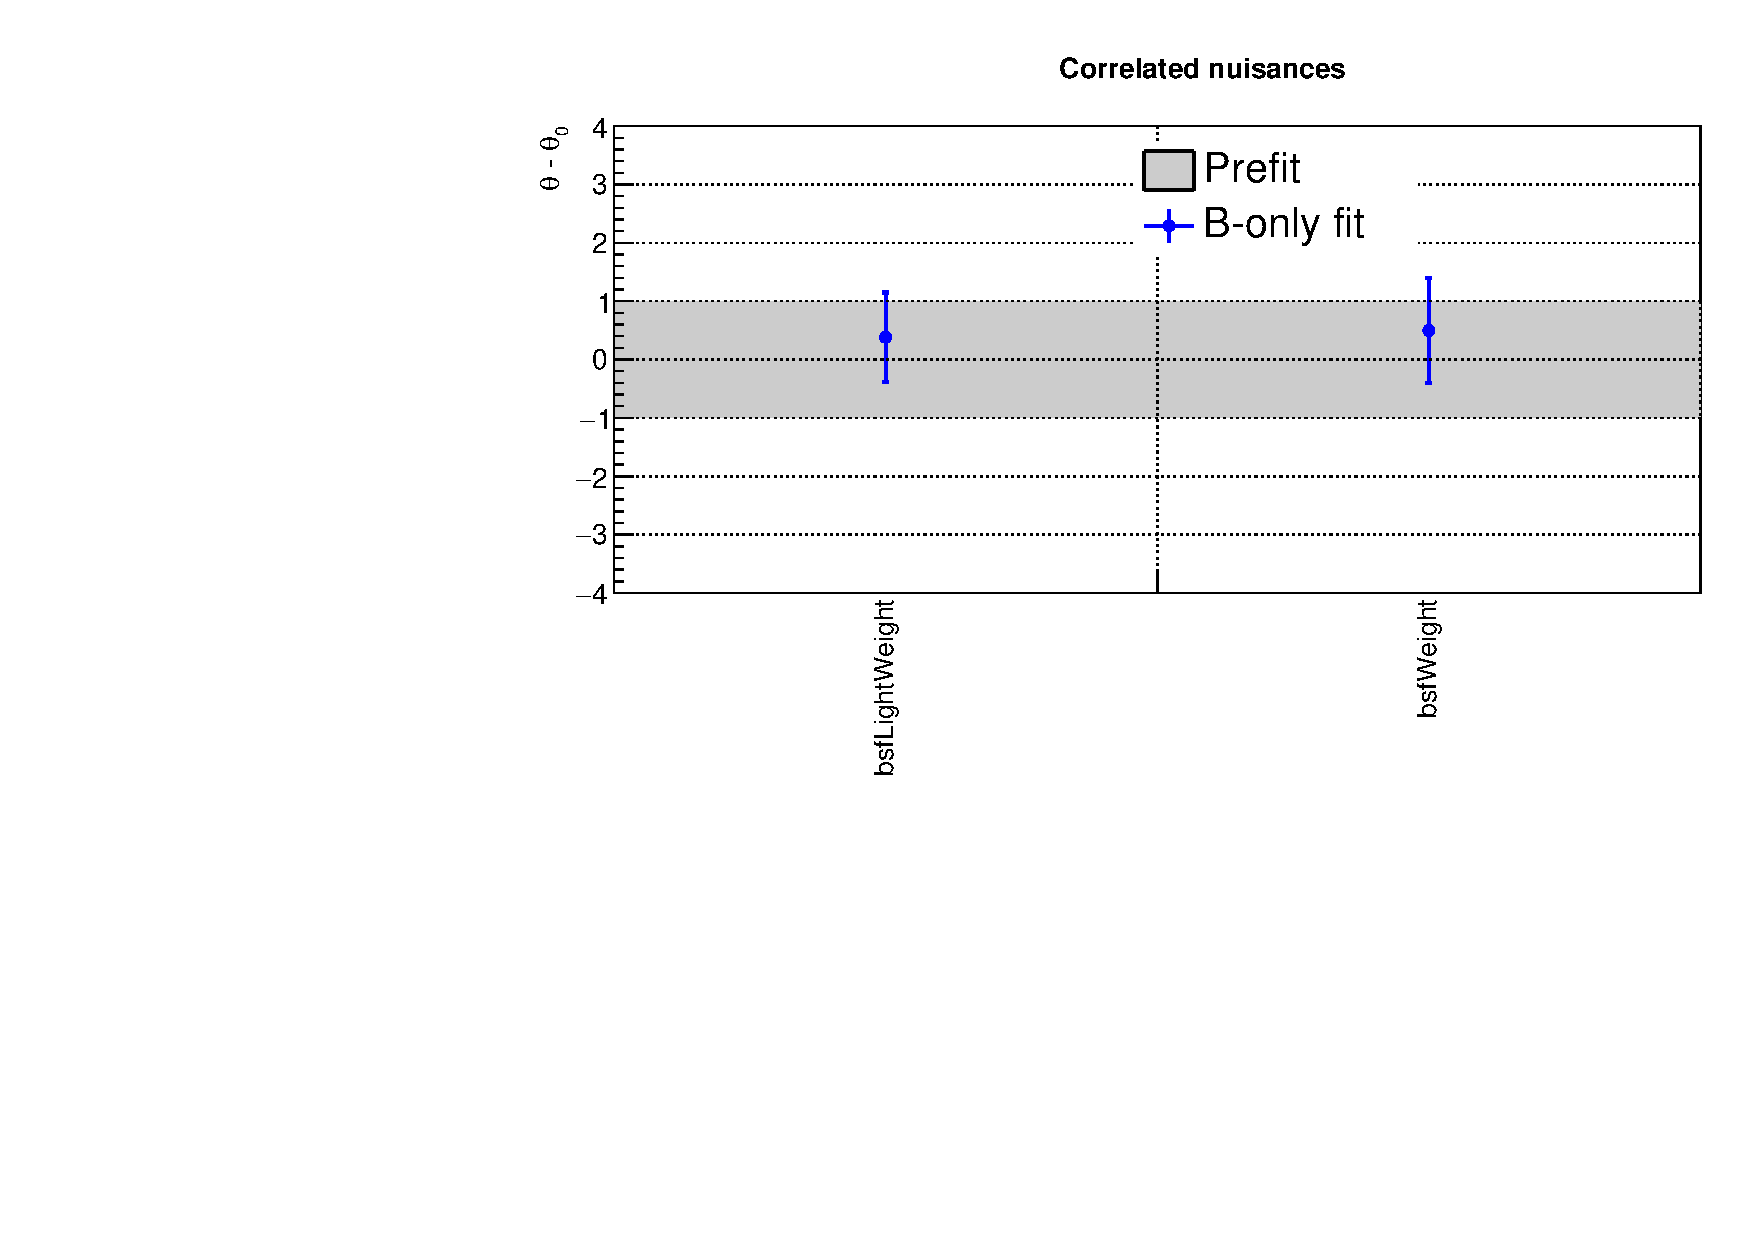
\includegraphics[width=0.6\textwidth]{figures/ZPlusbb/TemplateFitv1_HFXs0p5}
  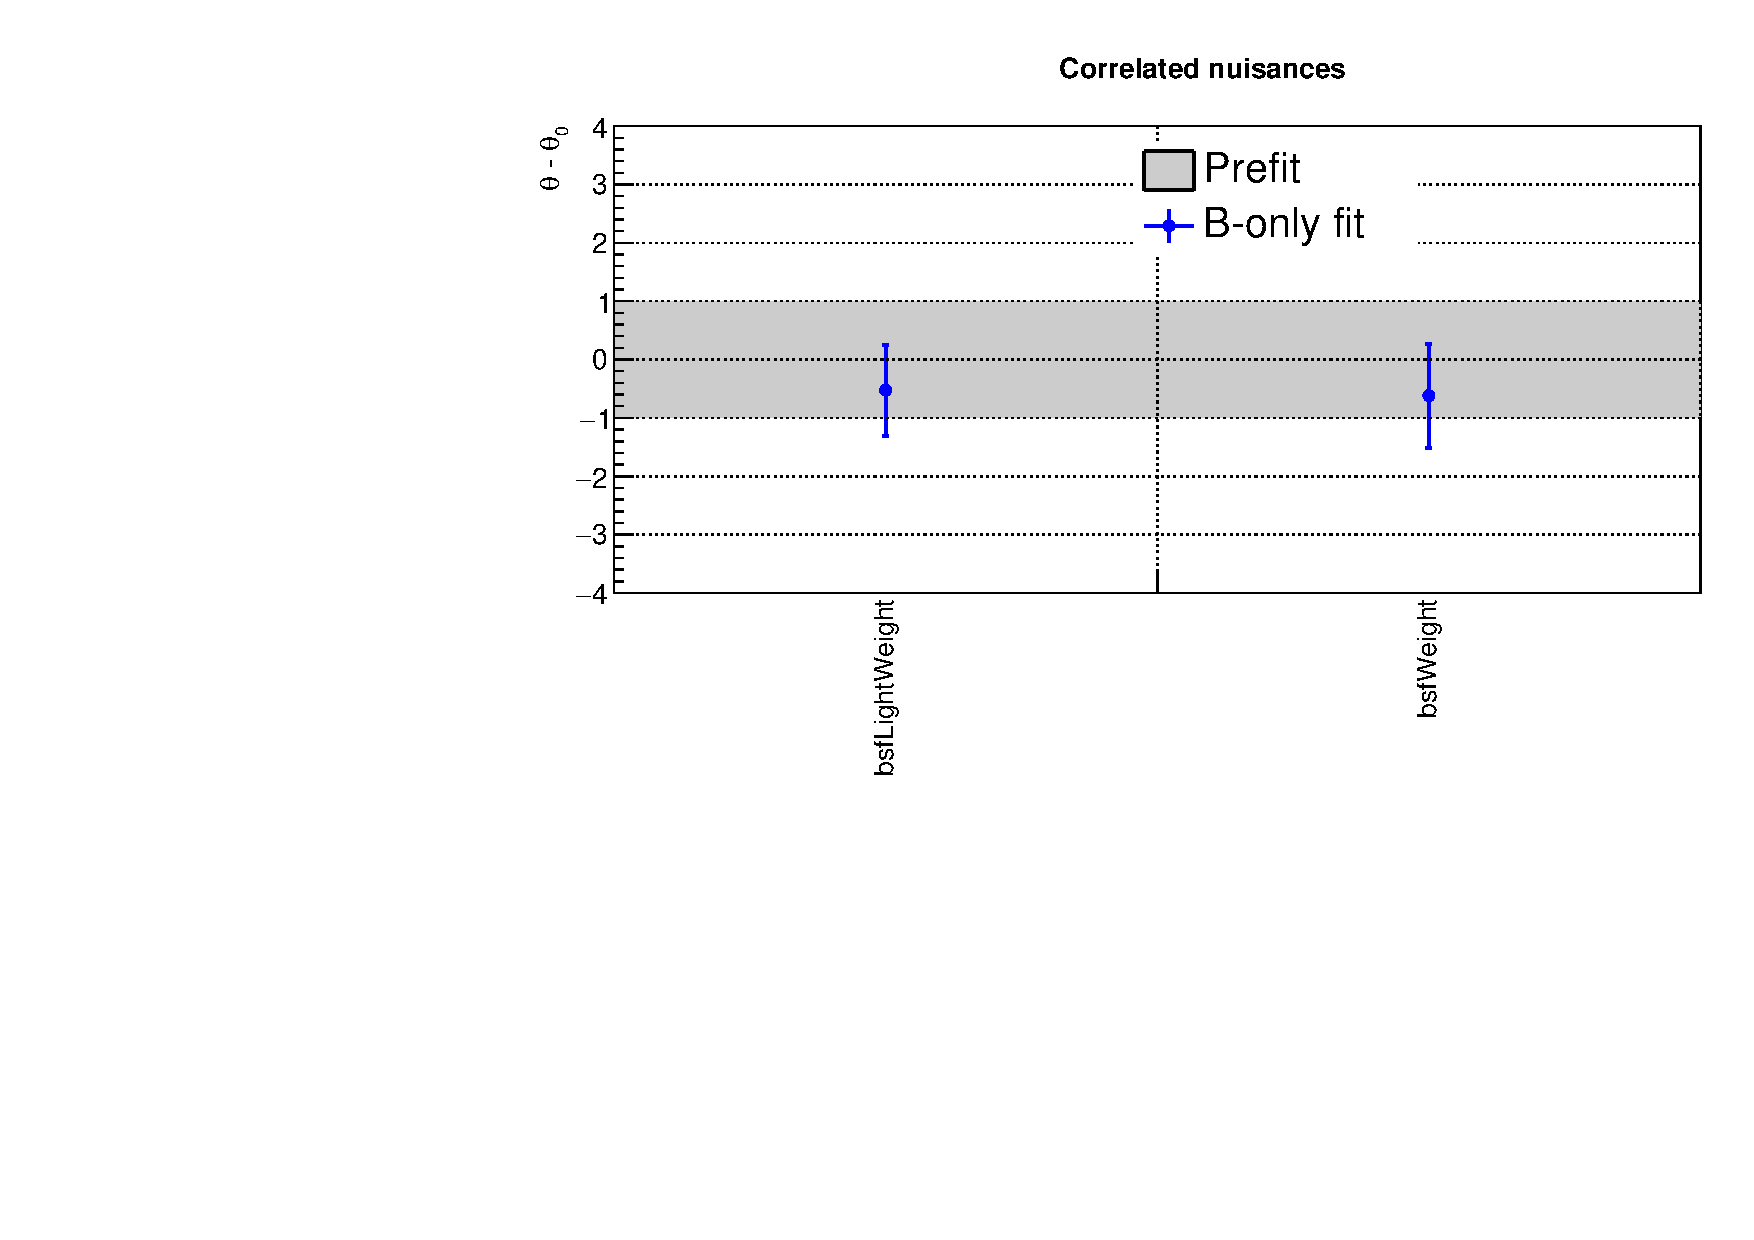
\includegraphics[width=0.6\textwidth]{figures/ZPlusbb/TemplateFitv1_HFXs2p0}
  \caption{\label{fig:btagsfge1b} Post-fit nuisances of a likelihood
    fit to data in the \mmj control region with scaling the cross section of heavy 
    flavour process by a factor of 0.5 (top) and 2.0 (bottom). }
  \label{fig:zplusbb}
\end{figure}

Another test which extracts the cross section of heavy flavour process is carried out 
with \mmj control sample. A likelihood is constructed with all known experimental and 
theoretical uncertainties in the analysis, unconstrained parameters per (\njet,\scalht) 
category to correct the normalisation of \zmmj with $\nb = 0$ and \ttj, and one 
unconstrained paramter to correct the cross section of \zmumuj with $\nb \geq 1$. Two separate 
fits are carried out with full dataset and G-H dataset. The extracted cross sections are 
$1.56 \pm 0.40$ and $1.10 \pm 0.46$ respectively.

\begin{figure}[h!]
  \centering
  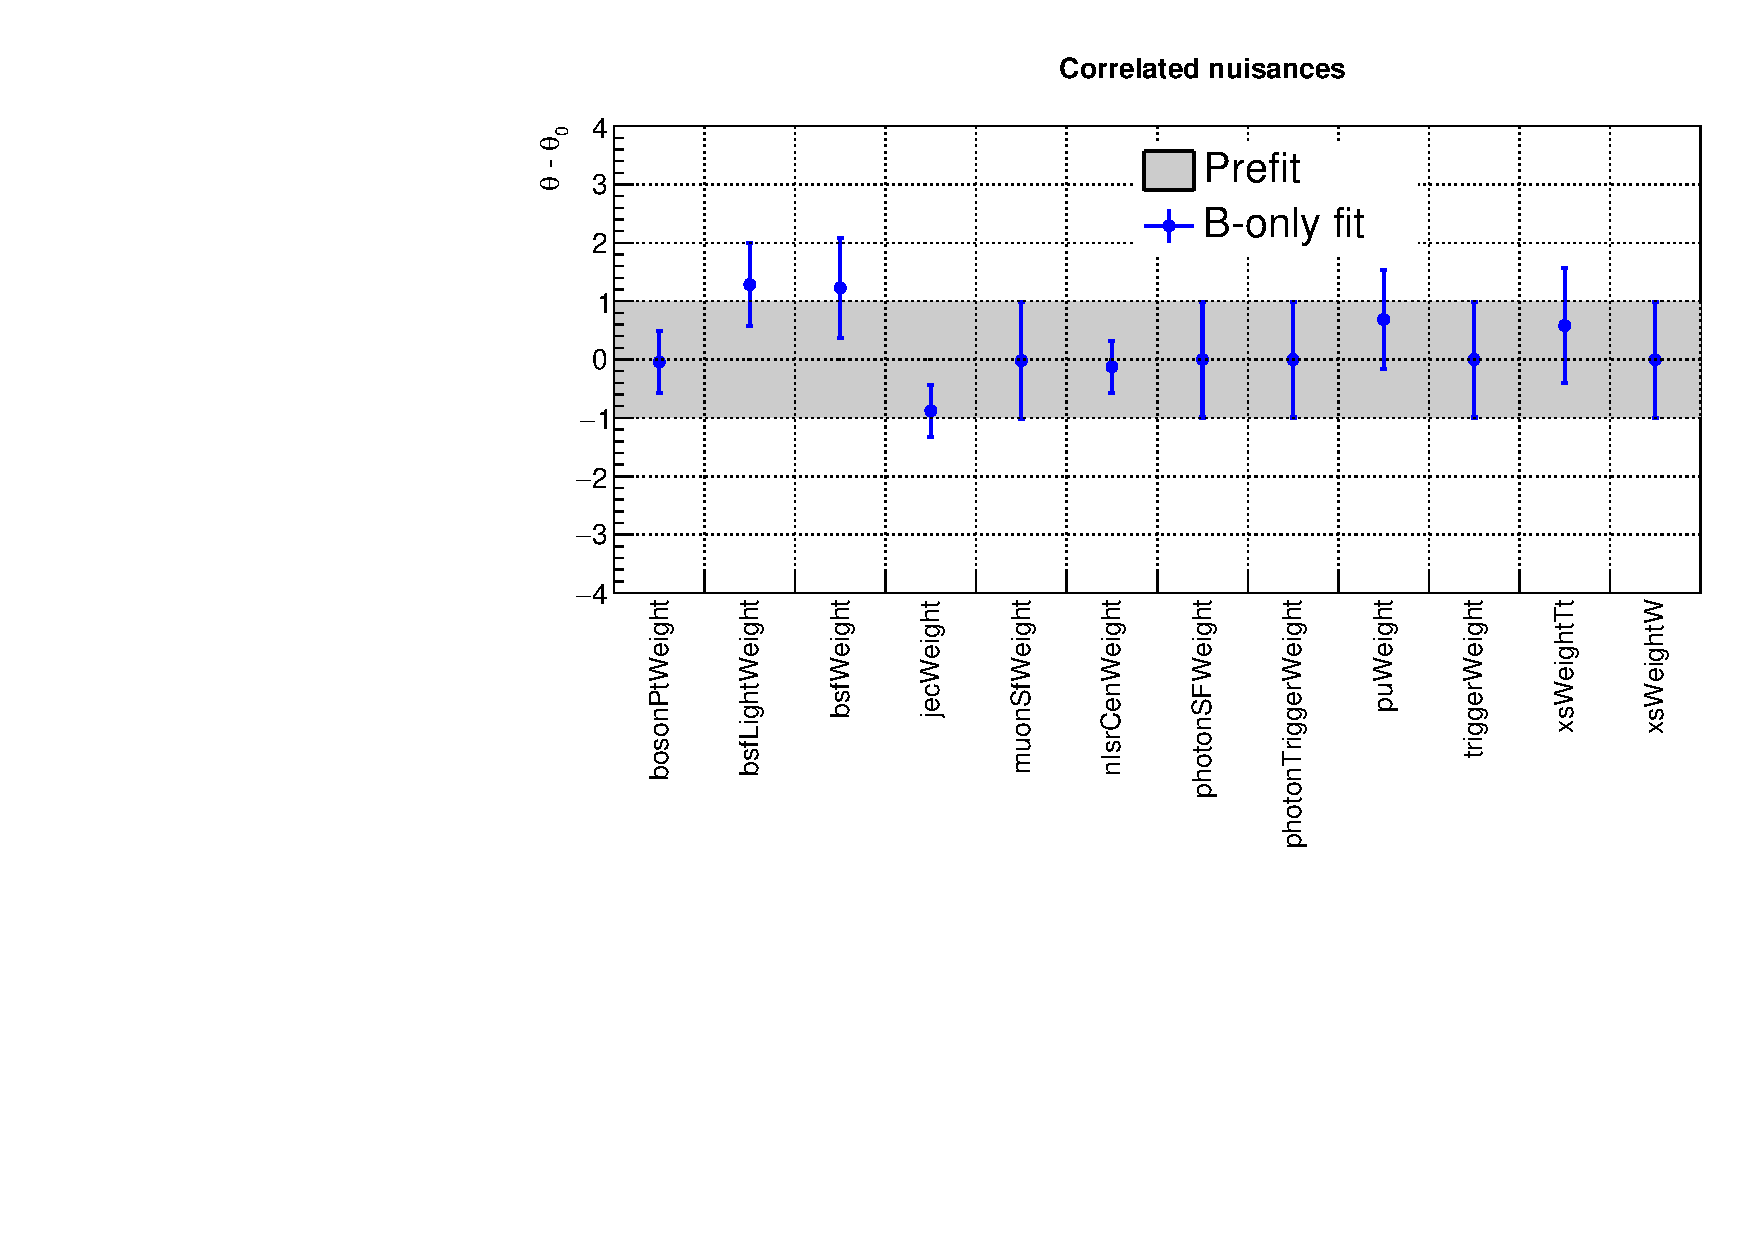
\includegraphics[width=0.6\textwidth]{figures/ZPlusbb/TemplateFitv2_36invfb}
  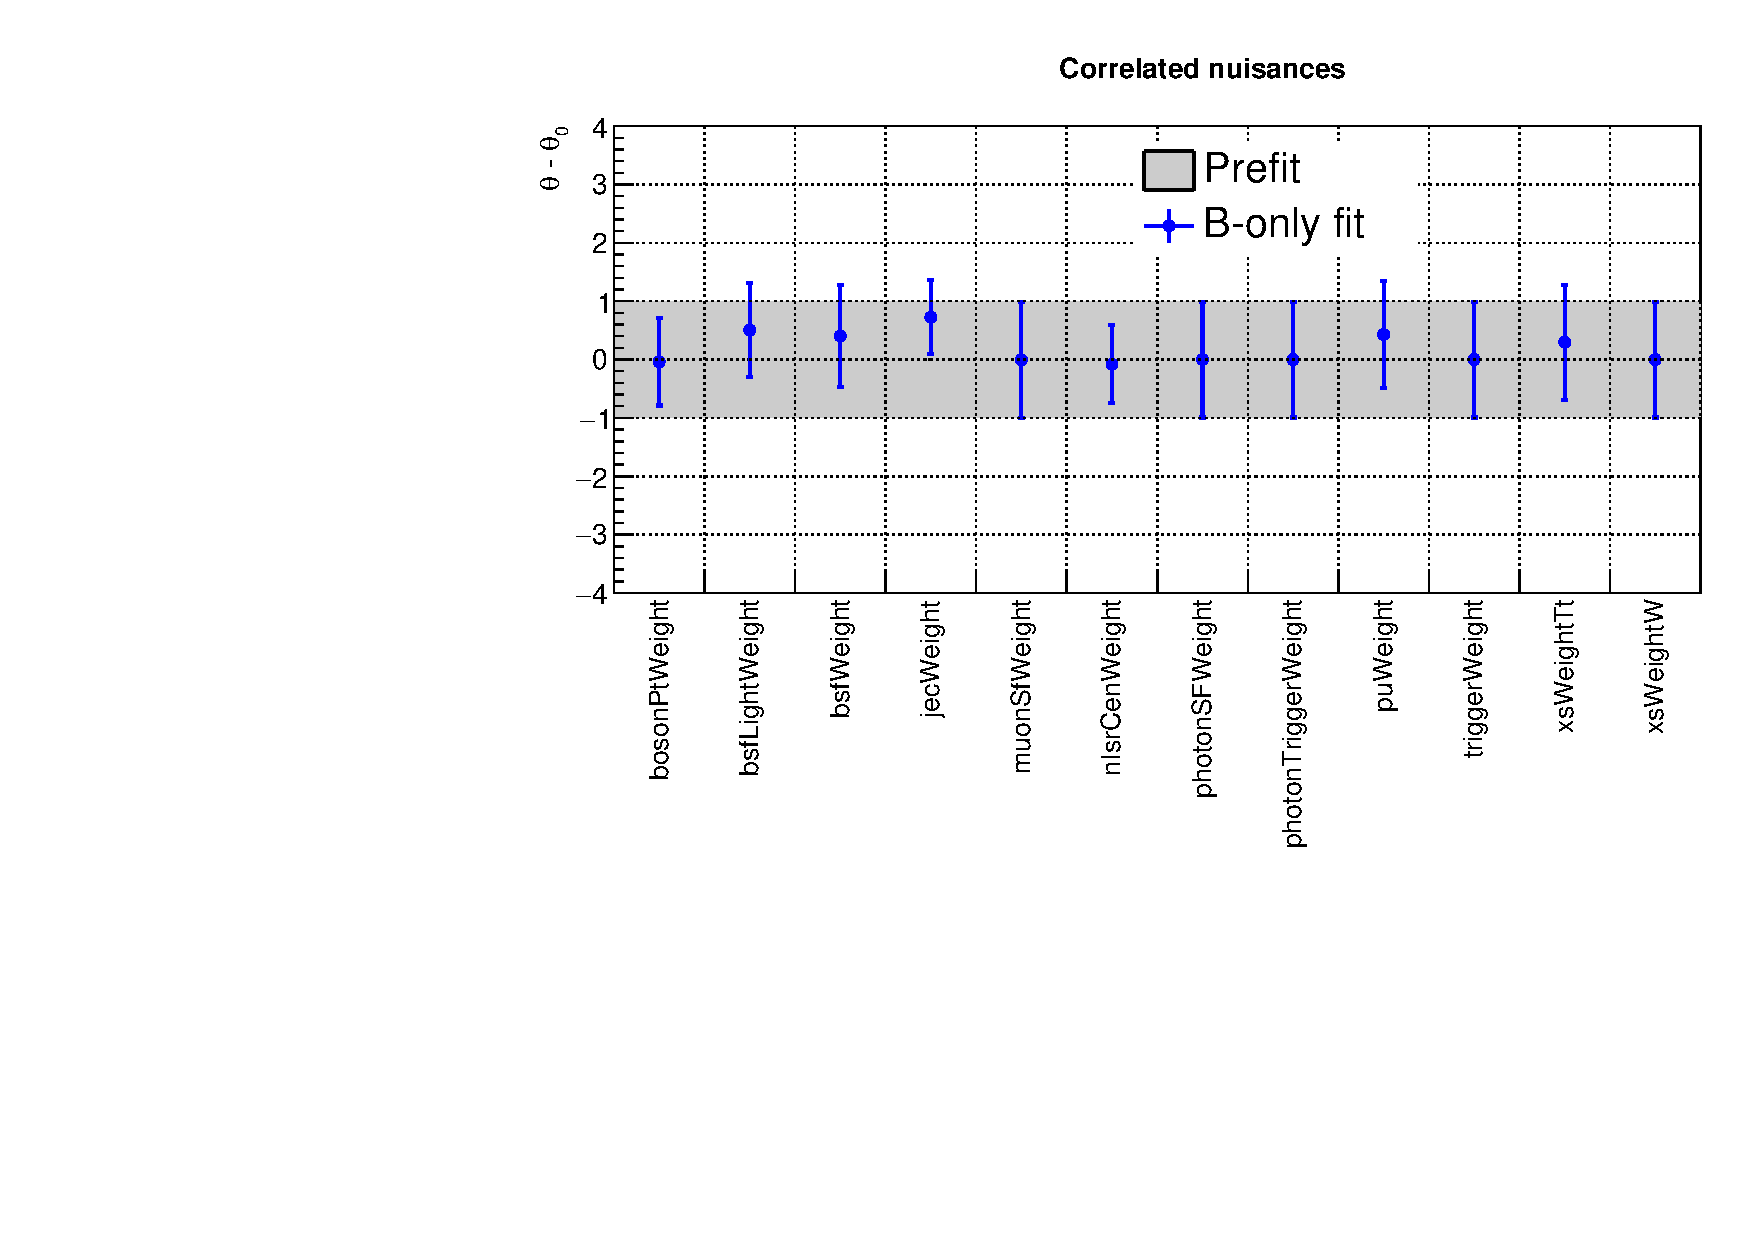
\includegraphics[width=0.6\textwidth]{figures/ZPlusbb/TemplateFitv2_16invfb}
  \caption{\label{fig:btagsfge1b} Post-fit nuisances of likelihood
    fits to data in the \mmj control region to extract heavy flavour 
    cross section, with full dataset with 35.9 \ifb (top) and partial dataset 
    G-H with 16.6 \ifb (bottom).}
  \label{fig:zplusbb2}
\end{figure}

